\section{銀河}

夜空に輝く星は,ほとんどが私たちの住む銀河系の星々である.しかし,ひとたび銀河系を離れて広大な宇宙を丹念に観測すると,そこには銀河の世界が広がっている.この宇宙には1000億個もの銀河が存在しており,銀河を理解することは,宇宙そのものの理解にもつながる.

\subsection{銀河の種類と形態分類}

銀河は大別すると,可視光の青色波長帯であるBバンドの絶対等級で約-18等を境にして,それより明るい巨大銀河(giant galaxy)と,それより暗い矮小銀河(dwarf galaxy)に分けられる.矮小銀河の質量は$10^9 M_\odot$ ($M_\odot$ は太陽質量(\SI{2e+30}{kg})を表す)よりも小さい.矮小銀河は暗さのために,観測研究の対象としての歴史は巨大銀河に比べるとまだ浅い.ここではまず巨大銀河の形態分類について述べる.形態分類とは,銀河を見かけの形で分類することがある.ただし形態と銀河のさまざまな物理量には後で述べるように良い相関がある.したがって,形態分類は銀河に関連する物理過程を理解する上で一助となる.

\begin{figure}[htbp]
	\centering
	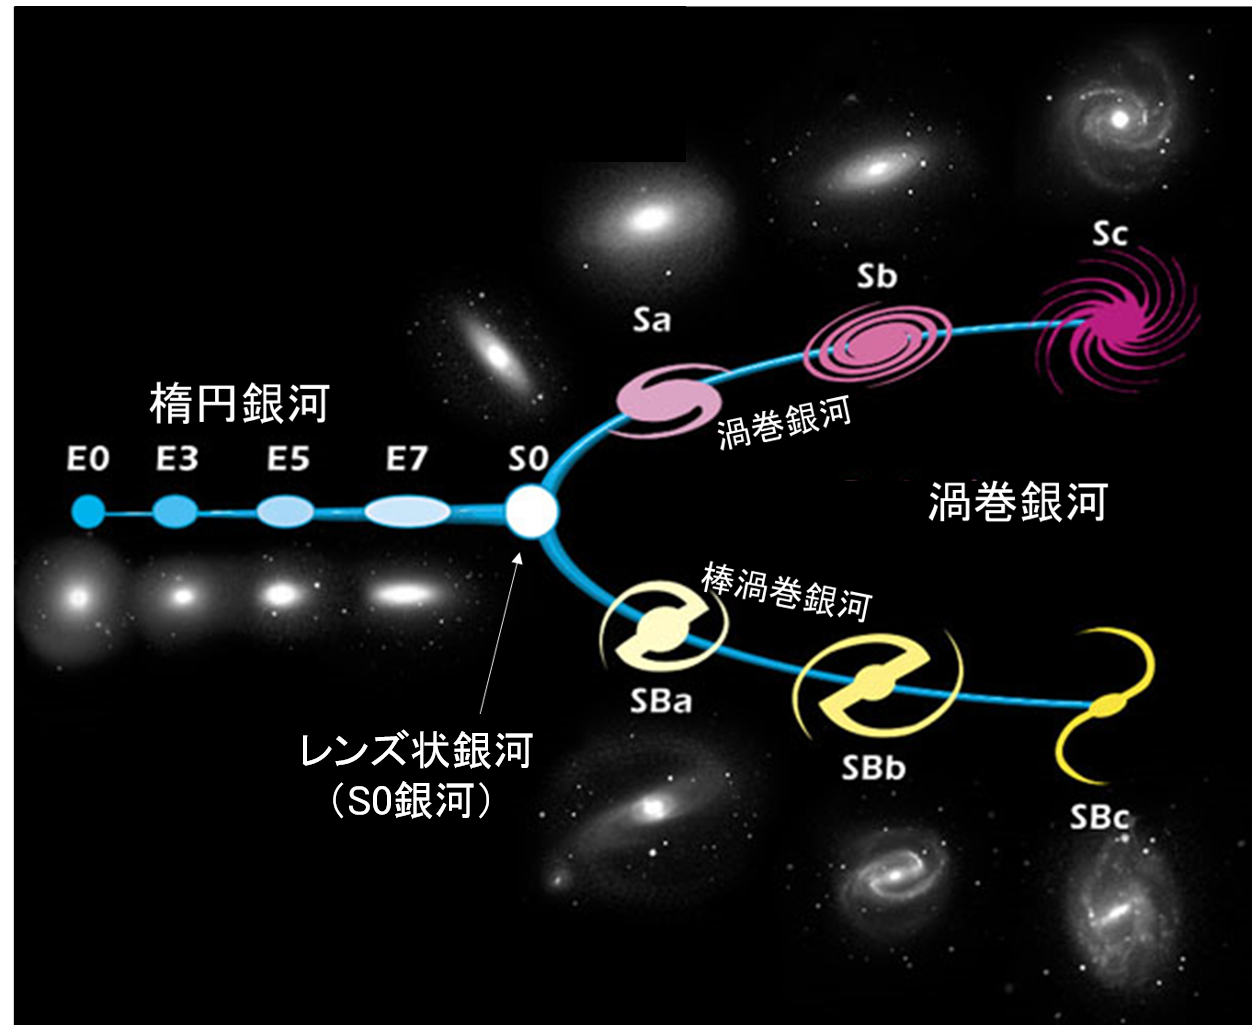
\includegraphics[width=0.7\linewidth]{pic/tuning-fork_diagram-2-2-1}
	\captionsetup{width=0.7\linewidth}
	\caption{ハッブルの音叉図に対応する実際の銀河.\citep{the_astronomical_society_of_japan__2017}より引用.}
	\label{fig:tuning-forkdiagram-2-2-1}
\end{figure}

\subsection{ハッブル分類}

巨大銀河の形態分の基本は,1936年にハッブル(E. Hubble)が提唱した,いわゆるハッブル分類である.ハッブルは,数100個の銀河を可視光の写真\footnote{当時使われていた写真乾板は,おもに青色の光に感度があるものであったため,正確には青色の波長帯で観測した写真ということになる.}を使ってグループ分けをした.大部分の銀河は回転対称性が良く,中心に光が集中した核を持つ規則銀河としてさらに詳細な分類を行ったが,2--3\%の銀河は不規則銀河であるとした,そして規則銀河を図\ref{fig:tuning-forkdiagram-2-2-1}に示すように,左側に楕円銀河(記号E),右側に通常の渦巻銀河(記号S,上の系列)と,中心に棒状構造のある棒渦巻銀河(記号SB,下の系列)を配置して分類した.図\ref{fig:tuning-forkdiagram-2-2-1}はハッブルの「音叉図」と呼ばれ,音叉図に示された左から右への形態の系列をハッブル系列という.

銀河が音叉図の左側にあるほど早期型(early type),右側にあるほど晩期型(late type)と呼ばれる.当時,楕円銀河のような渦巻腕のない銀河が進化をし,回転速度が増すにつれて赤道面からガスが吹き出して渦巻腕となってゆくとするジーンズ(J.H. Jeans)の星雲進化の仮説が流布していた.ハッブルは早期型と晩期型の分類を便宜上としているが,実際にはジーンズの仮説を意識していたようだ.ジーンズの仮説は現在では否定されているが,ハッブルの命名した早期型,晩期型という言葉は現在でも使用されている.その際にはたとえば,Sa型銀河はSb型銀河よりも早期である,という具合に図上での左右の相対関係で使われることもあれば,銀が全体の中で楕円銀河とS0銀河を早期型銀河と総称して使う場合もある.



\input{starburst_galaxy}

\subsection{渦巻銀河}

渦巻銀河は記号Sの後にa, b, cをつけて分類される.可視光で見た渦巻銀河はバルジと呼ばれる中心の回転楕円体状の成分と広がった円盤成分からなる.円盤では回転運動が卓越しているが,バルジではランダムな運動が卓越している.円盤ではガスや塵が多く,星形成活動が活発である.このガスと塵,およびそれから生まれたばかりの若い星は円盤の赤道面の薄い層に強く集中しており,渦巻腕として顕著に見える.

また密度が大変低いので通常の画像では見えにくいが,円盤よりもさらに遠くまで広がり,ほぼ球状に分布しているハローと呼ばれる成分がある.ハローの星もランダムな運動をしている.バルジとハローをあわせて回転楕円体成分と呼ぶことがあり,どちらも比較的古い星が主体となっている.たとえば球状星団は年齢の古い星団であるが,おもにハローに分布している.これに対して比較的若い星団であるが,おもに円盤に分布している.

渦巻銀河では,早期型(Sa)から晩期型(Sc)に向かうに従い,次に示すように性質が変化する.

\begin{enumerate}[(1)]
	\item 円盤の明るさに対するバルジの明るさの比が小さくなる.
	\item 渦巻腕の巻き込みの度合いが緩やかになる.
	\item 円盤で巨大な電離水素領域(HII領域)や若い明るい星と星団が目立ってくる.
	\item 星に対するガスや塵の相対質量が大きくなる.
\end{enumerate}

渦巻銀河は,大きく分けて普通の渦巻銀河と棒渦巻銀河に分かれる.棒渦巻銀河の割合は,およそ20\%--30\%であるが,詳しく調べると大部分の渦巻銀河には多少とも棒状構造が見られ,顕著な棒状構造のあるものを棒渦巻銀河ろ呼んでいる.したがって棒渦巻銀河と普通の渦巻銀河に大きな性質の差があるとは考えない方が良い.棒状構造は銀河同士の相互作用などでも生じると考えられるが,銀河に内在する要因によって次第に成長するという説もあり,成因はまだ十分に理解されていない.